\documentclass[final,t]{beamer}
\mode<presentation>
{

  \usetheme{PH}
}
% additional settings
\setbeamerfont{itemize}{size=\normalsize}
\setbeamerfont{itemize/enumerate body}{size=\normalsize}
\setbeamerfont{itemize/enumerate subbody}{size=\normalsize}

%additional packages
\usepackage{times} 
\usepackage{amsmath,amsthm, amssymb, latexsym}
\usepackage{exscale} \boldmath 
\usepackage{booktabs, array}
\usepackage{rotating} %sideways environment 
\usepackage[english]{babel}
\usepackage[latin1]{inputenc}
\usepackage{xspace}
\usepackage{url}
\usepackage{hyperref}
\usepackage{multicol}
\usepackage{xspace}
\usepackage{natbib}
\usepackage{subfig}
\usepackage[orientation=landscape,size=a0,scale=0.85]{beamerposter}
\usepackage{Sweave}

% To produce both postscript and pdf graphics, remove the eps and pdf
% parameters in the next line. Set default plot size to 5 x 3.5 in.

%\listfiles
%\graphicspath{{figures/}}
% Display a grid to help align images
%\beamertemplategridbackground[1cm]

\title{Dynamic modeling the neonicotinoid insecticide (imidacloprid) exposure risk for honeybees population}
\author[1]{Nan-Hung Hsieh$^1$, Chung-Min Liao$^2$}
\institute[1]{$^1$Department of Veterinary Integrative Biosciences, Texas \& University, College Station, TX\\
$^2$Department of Bioenvironmental Systems Engineering, National Taiwan University, Taipei, Taiwan}

%%%%%%%%%%%%%%%%%%%%%%%%%%%%

\begin{document}
\Sconcordance{concordance:beamerpostertest.tex:beamerpostertest.Rnw:%
1 45 1 1 18 26 1 1 13 1 9 11 0 1 2 30 1 1 88 2 4 1 1 2 4 4 1 2 4 2 1 2 %
4 91 1}


\begin{frame}[fragile]
  \begin{columns}[t]

    %-- Column 1 ---------------------------------------------------
    \begin{column}{0.19\linewidth}
      %-- Block 1-1
      \begin{block}{Introduction and Objectives}
Colony collapse disorder had become an ecology crisis for the honeybee population in recent years. Neonicotinoid insecticide is the suspected risk factor, which may accelerate the bee population decline. In there, the most widely used insecticide in the world is imidacloprid that can harm honeybees through their pollinating of nectar. This study has three main purposes:
        \begin{itemize}
          \item To develop an ecotoxicology-based population dynamic model and probabilistic risk assessment framework for honeybee colony.
          \item To assess the imidacloprid exposure-associated population decline in short, mid, and long-term time period. 
          \item To build the interactive web application to visualize the population dynamic and better understand the population exposure risk.
        \end{itemize}
      \end{block}
      
%-- Block 1-2
      \begin{block}{Study Flow Diagram}
Published toxicity bioassay of imidacloprid exposure and environmental investigations was be used as the study data.$^[^1^-^4^]$ The regression models were used to reconstruct a time-dependent dose-mortality profile. We also rebuilt the simple differential equation-based model that can be used to simulate the seasonal dynamic of the honeybee population and food storage according to the seasonality parameters.$^[^5^-^8^]$ This study parameterized the imidacloprid toxicity to simulate the toxicity effect to the honeybee population. 
      \begin{figure}[htb]
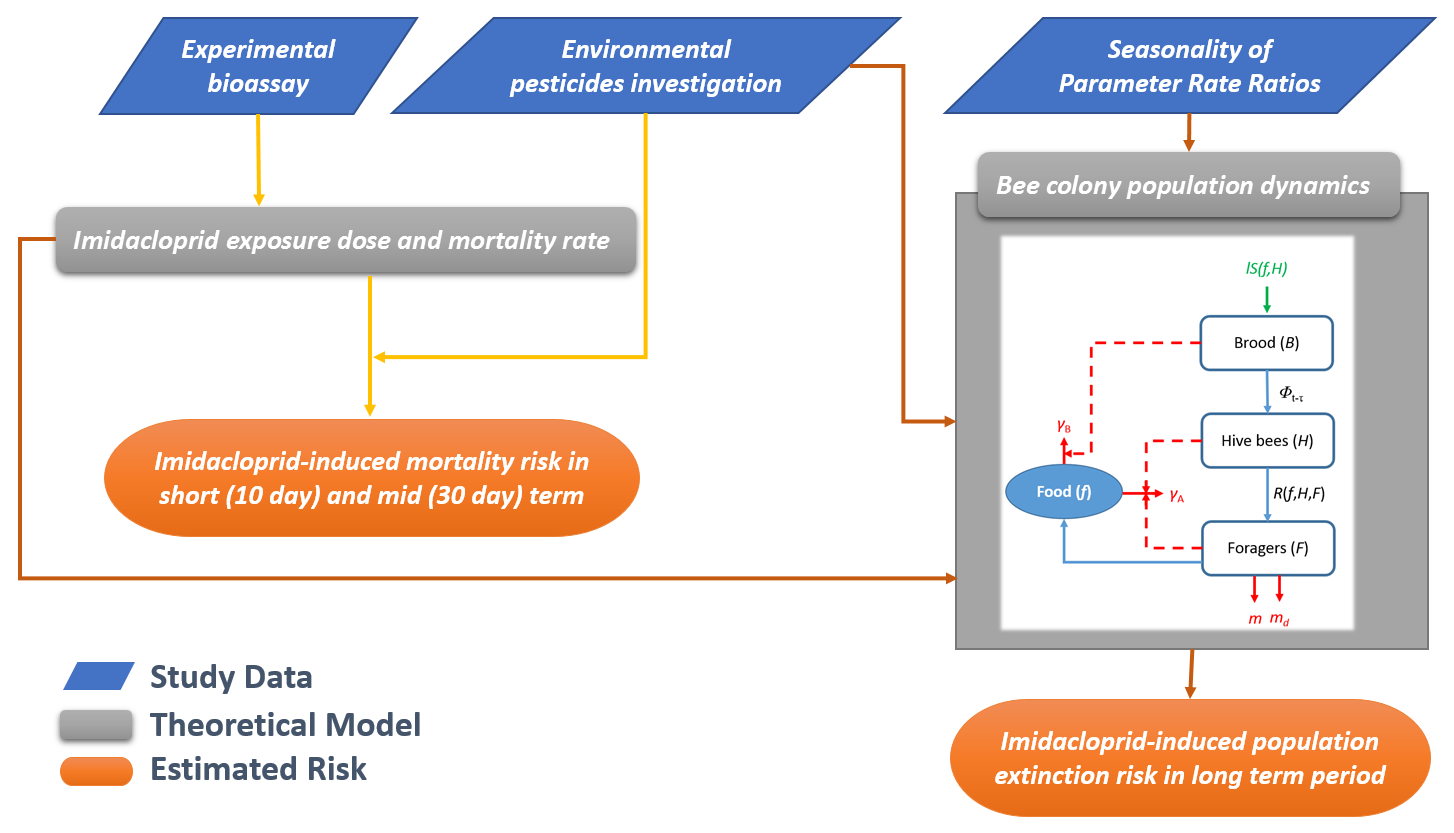
\includegraphics[width=.9\columnwidth]{flowchart.png}
\end{figure}
    \end{block}
    
%-- Block 1-4
\begin{block}{Systematic Modeling and Analysis Method}
R packages used in the mathematical model development and risk analysis\\
\\
% latex table generated in R 3.3.1 by xtable 1.8-2 package
% Thu Jan 12 21:51:43 2017
\begin{tabular}{lll}
  \hline
Tool & Description & Version \\ 
  \hline
desolve & General solvers for differential equation & 1.11-1 \\ 
  mc2d & Two-dimensional Monte-Carlo simulations & 0.1-15 \\ 
  fitdistplus & Choosing and fitting of univariate distributions & 1.0-6 \\ 
  sensitivity & Parameter sensitivity test for dynamic model & 1.12.2 \\ 
  EnvStats & Simulating of environmental imidacloprid distribution & 2.1.1 \\ 
   \hline
\end{tabular}\end{block}
      %-- Block 3-2
      \begin{block}{Populaion Dynamic Model}
        The model includes four compartments that are foragers ($F$), hive bees ($H$), broods ($B$), and food ($f$), respectively can be written as 
        \\
        \begin{equation}
          \frac{\mathrm{dF}}{\mathrm{dt}} \,= R(f,H,F)H-(m+m_d)F
        \end{equation}
        \begin{equation}
          \frac{\mathrm{dH}}{\mathrm{dt}} \,= \phi B(t-\tau)-R(f,H,F)H
        \end{equation}                
         \begin{equation}
          \frac{\mathrm{dB}}{\mathrm{dt}} \,= ls(f,H)-\phi B
        \end{equation}
        \begin{equation}
          \frac{\mathrm{df}}{\mathrm{dt}} \,= cF-\gamma_A(H+F)-\gamma_B B
        \end{equation}
        where $m$ is the forager natural death rate, $m_d$ is the imidacloprid-increased forager death rate, $\phi$ is the emergence rate, $\tau$ is the lag time of adult bees emerge from pupation, $c$ is the food collection rate (gram per forager per day), $l$ is the egg laying rate, $\gamma_A$ and $\gamma_B$ are the food consumption rate for adult bees and brood(gram per number of bee per day). In addition, the number of adult bees and broods can be influenced by the recruitment and survival function, respectively. That are
        \begin{equation}
          S(f, H)= (\frac{\mathrm{f^2}}{\mathrm{b^2+f^2}})(\frac{\mathrm{H}}{\mathrm{v+H}})
        \end{equation}
        \begin{equation}
          R(H, F, f)=\alpha_m_i_n+\alpha_m_a_x(\frac{\mathrm{b^2}}{\mathrm{b^2+f^2}})-\sigma(\frac{\mathrm{F}}{\mathrm{F+H}})
        \end{equation}
        where $b$ is the food impact constant and v is the hive bees impact constant, $\alpha_m_i_n$ and $\alpha_m_a_x$ are the minimum and maximum forager transition rate, and $\sigma$ is the social inhibition rate. The functions reflect that the limited food resources can stimulate hive bees to become foragers at a younger age, causing a precocious onset of foraging, and the way that brood survival declines when food stores are low.
      \end{block}
    \end{column}%1

    %-- Column 2 ---------------------------------------------------
    \begin{column}{0.16\linewidth}
      \begin{block}{Bioassay and Predictions}

        \begin{figure}[htb]
        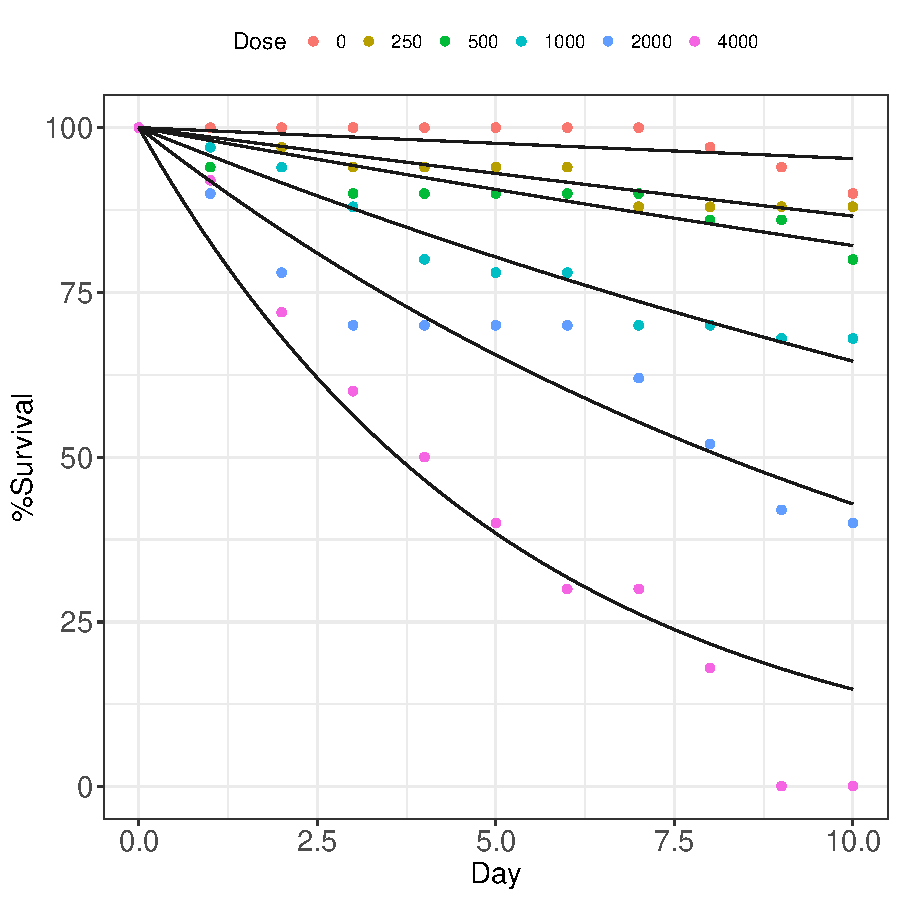
\includegraphics[width=.8\columnwidth]{beamerpostertest-fig1}
        \end{figure}
        \begin{figure}[htb]
        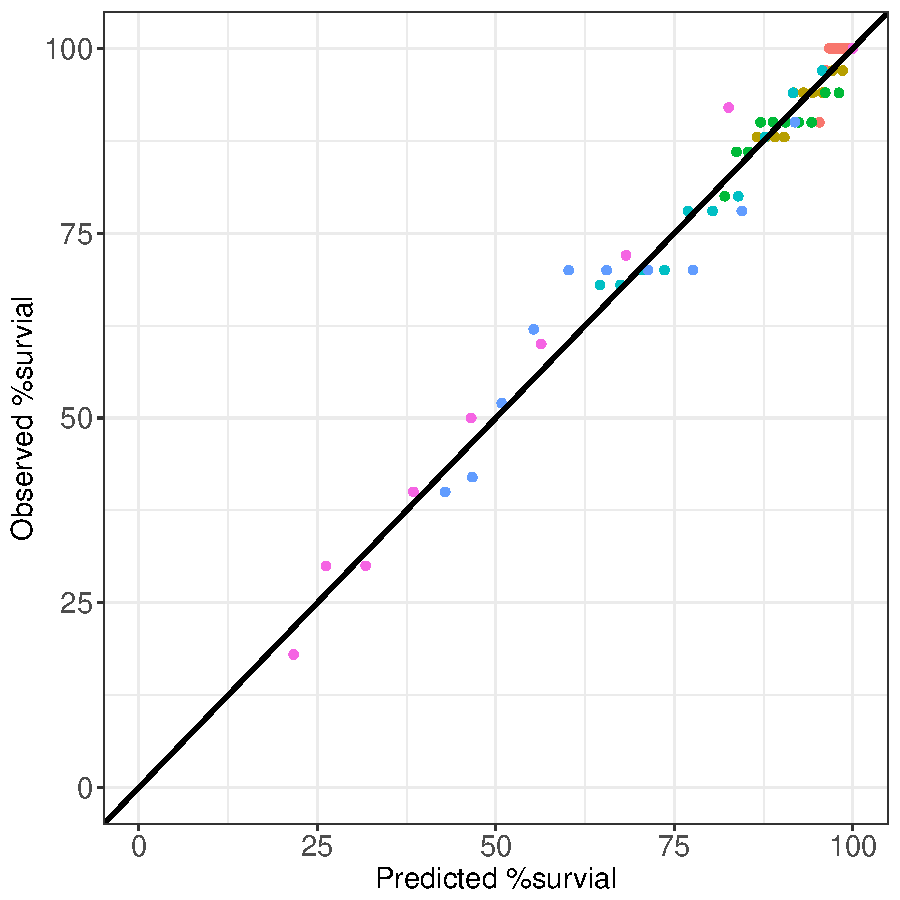
\includegraphics[width=.8\columnwidth]{beamerpostertest-fig2}
        \end{figure}
        The dynamic model predicted the time-dependent honeybees survival probability under different imidacloprid exposure doses. The calibration results are showing the high precision ($r^2$ = 0.99) in model performance.
        
        
        \begin{figure}[htb]
        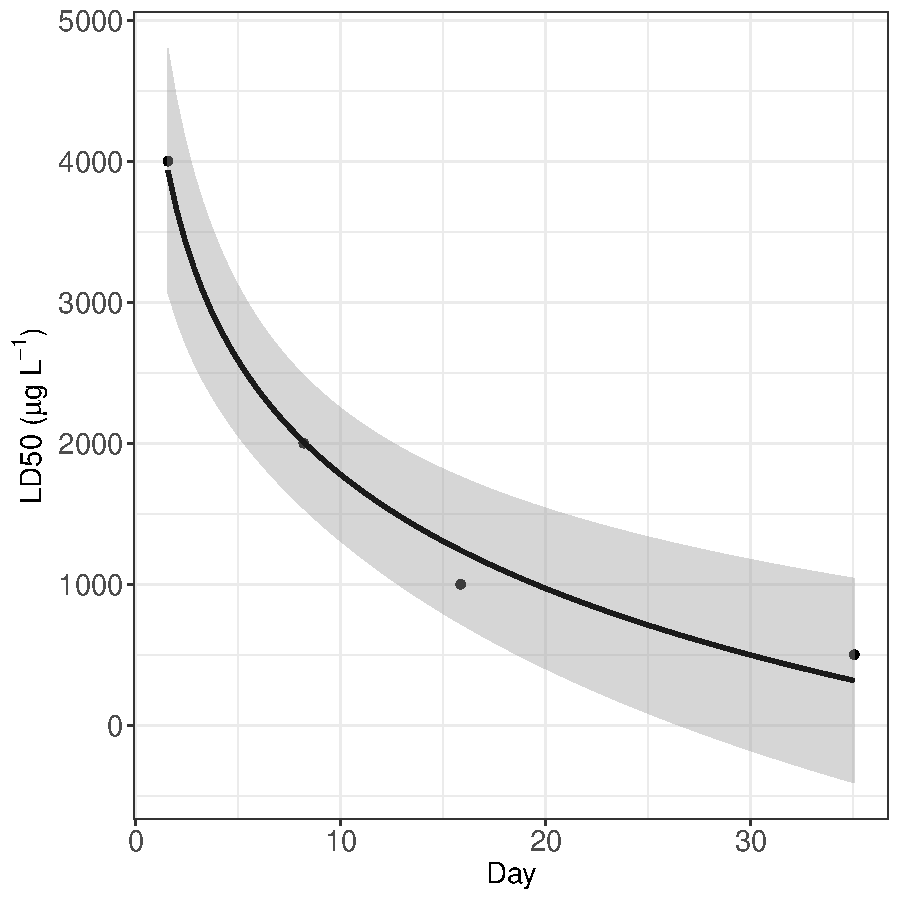
\includegraphics[width=.8\columnwidth]{beamerpostertest-fig3}
        \end{figure}
        
        \begin{figure}[htb]
        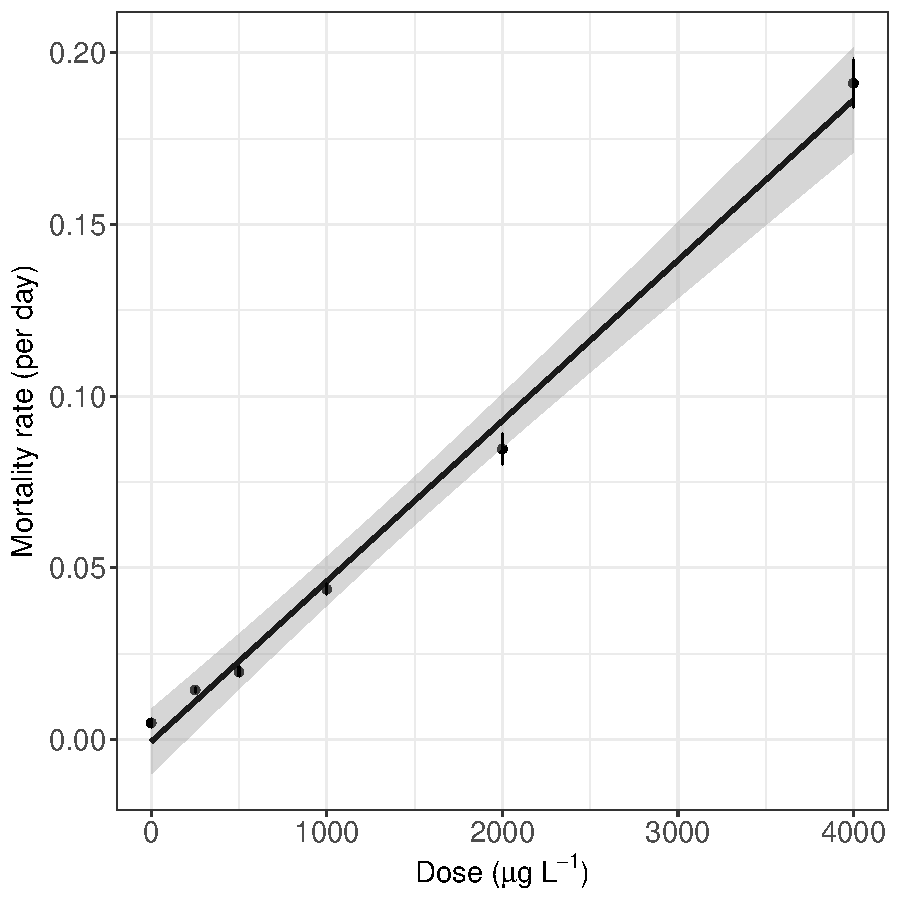
\includegraphics[width=.8\columnwidth]{beamerpostertest-fig4}
        \end{figure}
        Time-dependent LD50 with 95\% confidence interval to represent the exposure threshold and uncertainty. The dose-response profile for imidacloprid exposure-associated mortality rate was constructed to use in risk assessment.
      \end{block}
    \end{column}%2

    %-- Column 3 ---------------------------------------------------
    \begin{column}{0.24\linewidth}
      %-- Block 3-1
      \begin{block}{Predicted Environmental Exposure}
      
      \begin{figure}[htb]
      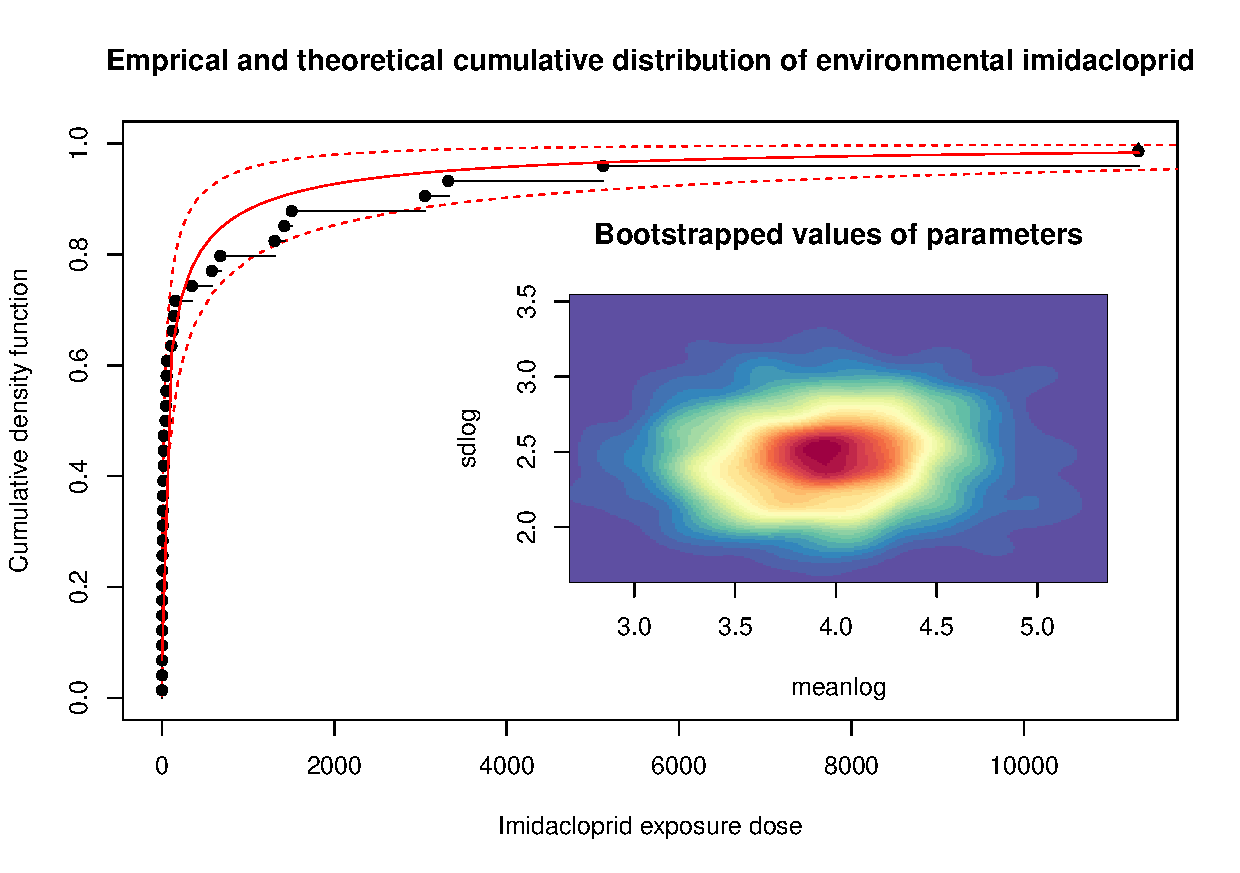
\includegraphics[width=.9\columnwidth]{fig3}
      \end{figure}
      The result of the fitting of a lognormal distribution to the environmental imidacloprid investigation dataset. For each value of the data, the cumulative density function is plotted to compare the empirical and theoretical results with 95 \% CI. A parametric bootstrap was used for the uncertainty around the meanlog and sdlog of the fitted lognormal distribution for the dataset.
      \end{block}

      %-- Block 3-2
      \begin{block}{Risk assessment for short- and mid-term exposure}
      \begin{figure}[htb]
      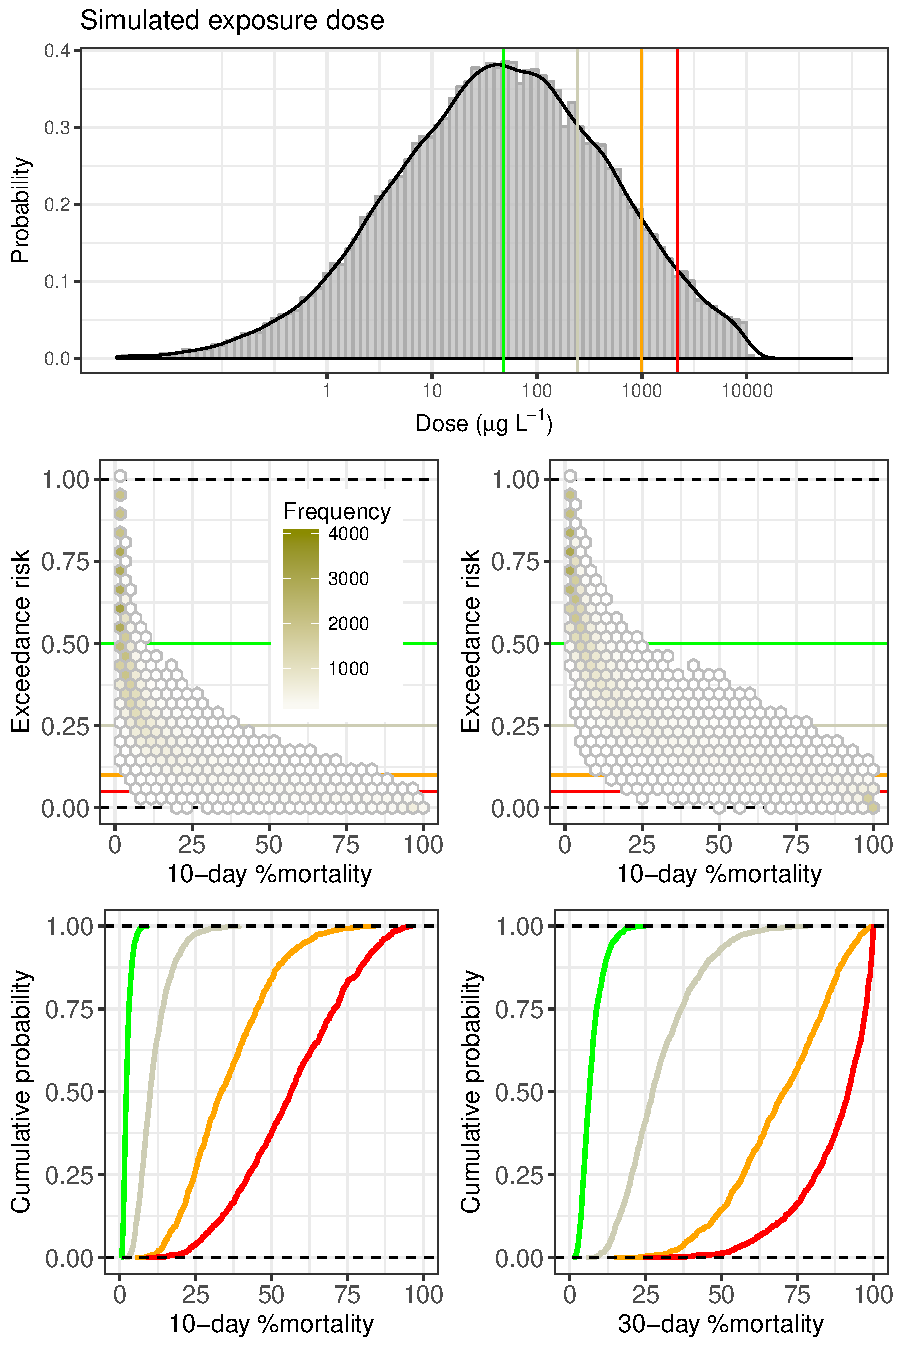
\includegraphics[width=.9\columnwidth]{fig4}
      \end{figure}
      Estimated risk of imidacloprid exposure-associated \%mortality of honeybees at exceedance probabilities of 0.5, 0.25, 0.1, 0.05, respectively, representing the conditions from medium to high exposure levels. Both simulating exposure and effect conditions were considered the variability and uncertainty to calculate the population risk. 
      \end{block}      
    \end{column}
    
    %4
    \begin{column}{0.38\linewidth}
      %-- Block 4-1
      \begin{block}{Risk assessment for long-term exposure}
      \begin{figure}[htb]
      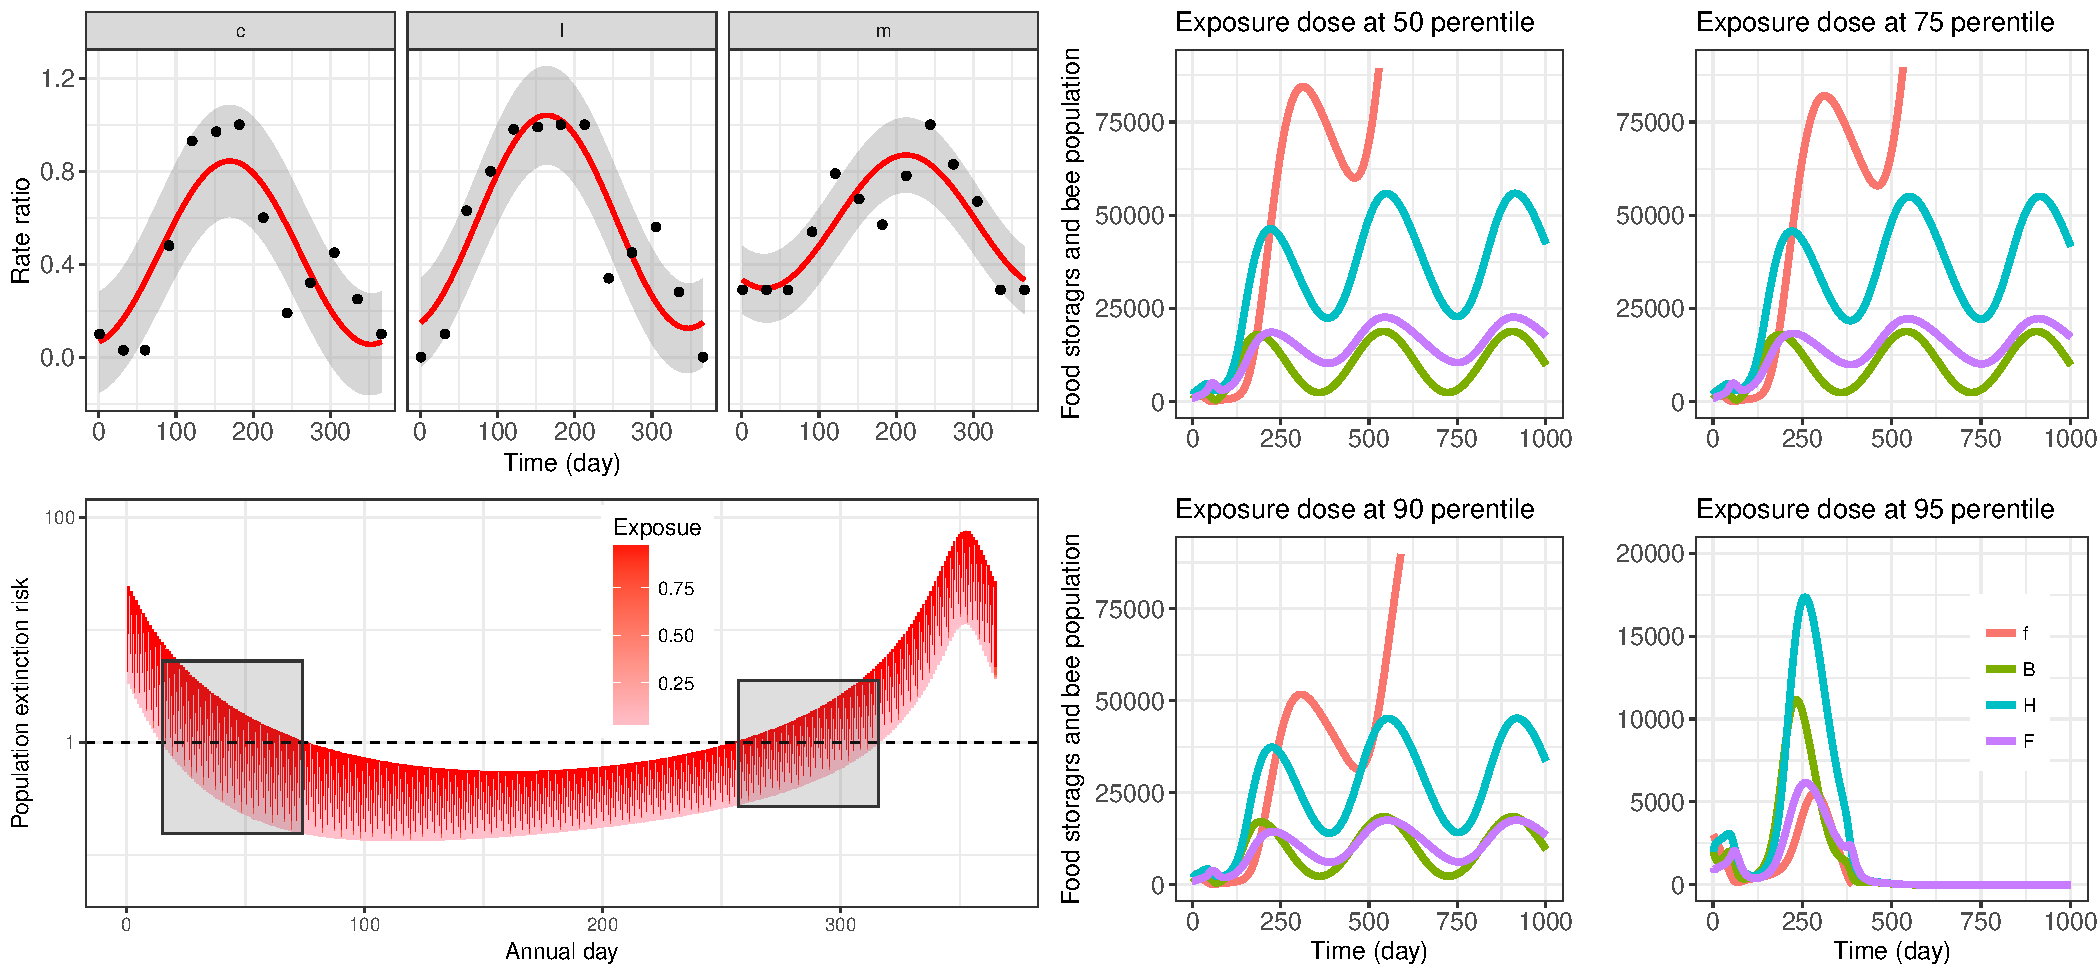
\includegraphics[width=.95\columnwidth]{fig5}
      \end{figure}
      Predicted results of seasonal variation of parameter rate ratios with 95 \% CI for food collection (c), egg laying (l), and mortality (m). According to the equilibrium solution of dynamic model, this study finds that the current imidacloprid exposure can affect the honeybees population in two time periods of the year, from late winter to early spring and autumn period. The food collection is also an important factor, which can affect the bee population in the winter. By using the dynamic simulation with predicted parameters, the bee population will go extinction when the exposure dose of imidacloprid exceed 2500 $\mu$g L$^-^1$. The user interface was successfully developed to visualize the population dynamics and find the critical threshold.
      \end{block}
      
%-- Block 4-2
      \begin{block}{Sensitivity Analysis}
      \begin{figure}[htb]
      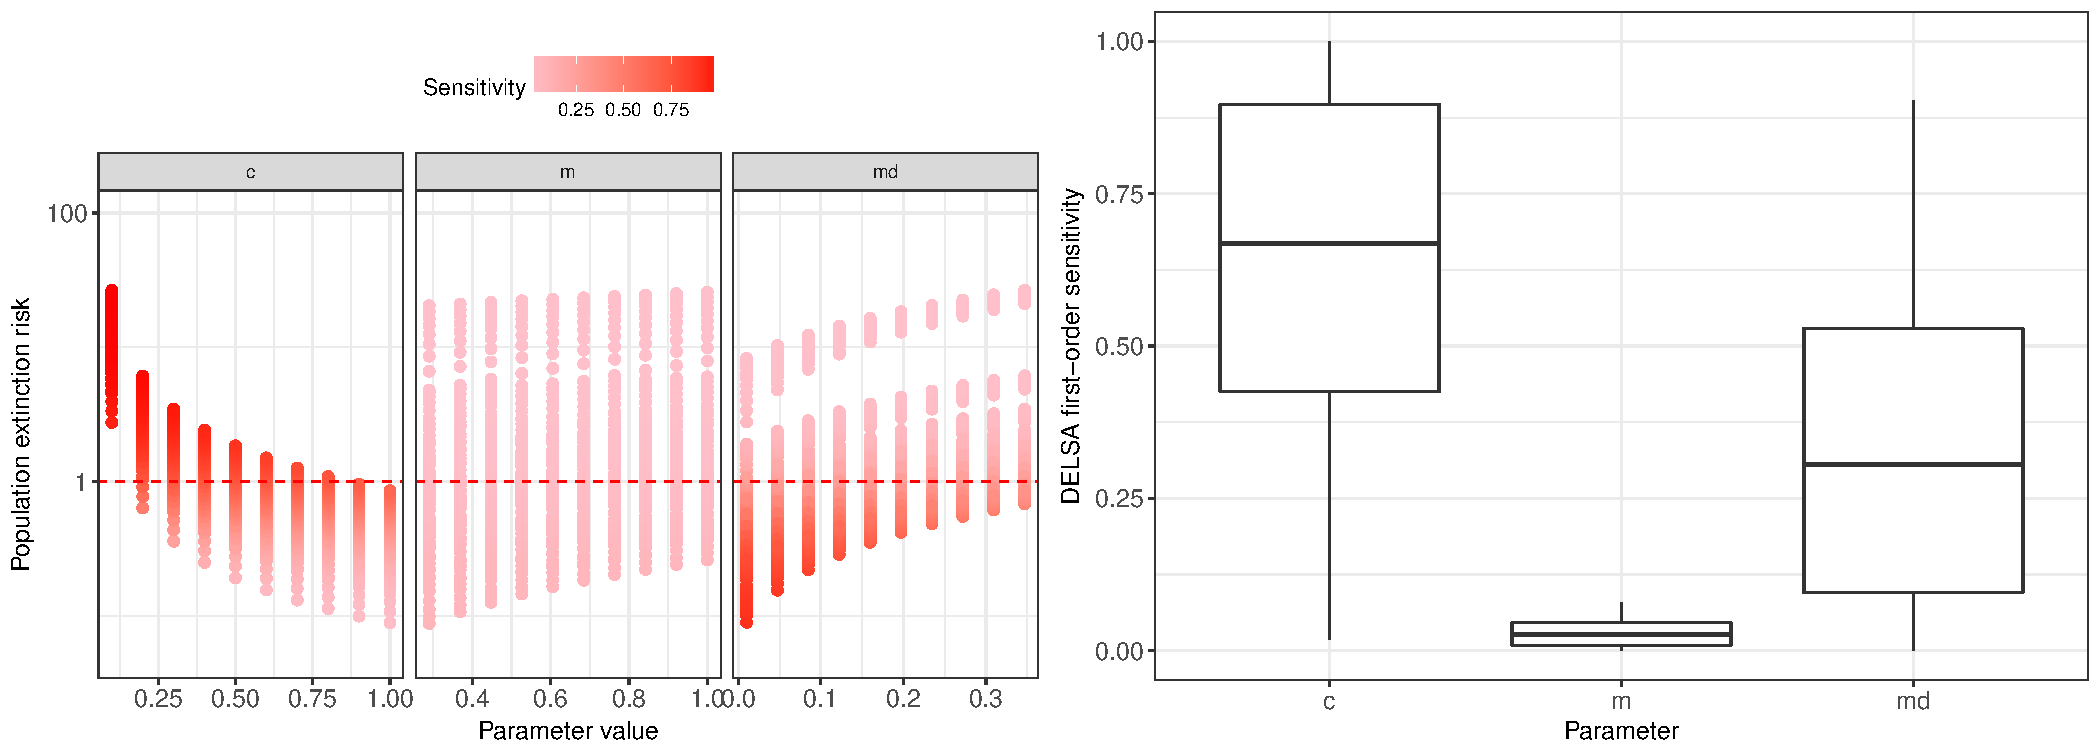
\includegraphics[width=.95\columnwidth]{fig6}
      \end{figure}
      Distributed evaluation of local sensitivity analysis (DELSA) tests the food collection (c), natural mortality (m), and imidacloprid-increased mortality rate (m$_d$) across the parameter space. The result shows that imidacloprid can determine the honeybees extinction in our estimated range. However, food collection plays the most important role to determine the extinction of bee colony.
      \end{block} 
      
%-- Block 4-3
      \begin{block}{Conclusions}
        \begin{itemize}
          \item This study established the population risk assessment framework by considering the uncertainty and variability in model predictions.
          \item According to the current results of the risk evaluation, the realistic in-field exposure dose distribution of imidacloprid can only impact the honeybees population slightly.
          \item We hope that our constructed interactive web application can help people better understand the toxicity effect on honey bee population in risk communication.
        \end{itemize}
		\end{block}

      \begin{block}{Acknowledgements}
      The authors appreciate the useful discussion and suggestion from the members of Biosystem Modeling and Control Lab in National Taiwan University.

		\end{block}

%-- Block 4-4
 \begin{columns}[onlytextwidth, t]
\column{0.62\linewidth}
      \begin{block}{Bibliography}
        \begin{itemize}
          \item 1. DEFRA (2007) Project no.PS2322.
          \item 2. Cresswell (2011) Ecotoxicology. 20:149-57.
          \item 3. Greenpeace (2014) The Bees' Burden.
          \item 4. Greenpeace (2014) A Toxic Eden.
          \item 5. Perry et al. (2015) PNAS. 112:3427-32.
          \item 6. Henry et al. (2016) Apidologie. doi:10.1007/s13592-016-0476-0 
          \item 7. Russell et al.(2013) Ecol Model. 265:158-169.
          \item 8. Khoury et al.(2013) PLOS ONE. 8: e59084. 
        \end{itemize}
		\end{block}

\column{0.36\linewidth}
    \begin{block}{QR code}
    The poster pdf and interactive user interface (UI) are show as following 
        \begin{figure}[h]
 \centering
  \subfloat[Poster pdf\label{fig:a}]{
\includegraphics[height=4cm,width=4cm]{UI.png}}\qquad
  \subfloat[UI\label{fig:b}]{
\includegraphics[height=4cm,width=4cm]{UI.png}}
\end{figure}
    \end{block}
\end{columns}
% 
    \end{column}%3
  \end{columns}

\end{frame}
\end{document}


